\section{\textsf{Introduction to Vectors}}
In mathematics, a vector is a list of elements. A single element on its own is known as a scalar. A vector is basically a one-dimensional array of elements.

With GLM, you can create a vector as follows:

\begin{frame}{}
    \begin{figure}[ht]
    \centering
    \colorbox{backgroundcolor}{
        \parbox{0.9\textwidth}{
            \lstinputlisting[language=csh,style=csharp]
            {code/chap2_MathematicsPrinciples/CreatingAVector.cpp}
        }
    }
    \caption{GLM test snippet}
    \label{fig:creatingAVector}
    \end{figure}
\end{frame}

Vectors can be of any size, but in graphics programming, only vectors of sizes 2 to 4 are commonly used, so those are the only ones included in GLM.

Mathematic notation for vectors is as follows:

\begin{equation*}
    \vec{v} =\begin{pmatrix}
    0\\
    0\\
    0
    \end{pmatrix}
\end{equation*}

In order, a vector's elements can be referred to as: X, Y, Z, and W. X, Y, and Z are positions in 3D space. W is different; it is known as the \textbf{homogeneous vertex coordinate}. It isn't important for now, but will be discussed later.

So, what can you do with a vector? Let's start with basic vector arithmetic.

\subsection{\textsf{Scalar operations}}
Scalar operations refer to any operation that uses both a scalar (a single element) and a vector (multiple elements). Simply put, the scalar is applied to each element of the vector separately. For example:

\begin{equation*}
\begin{pmatrix}
2\\
1\\
0
\end{pmatrix} +3=\begin{pmatrix}
2+3\\
1+3\\
0+3
\end{pmatrix} =\begin{pmatrix}
5\\
4\\
3
\end{pmatrix}
\end{equation*}

It works exactly the same for subtraction, multiplication, and division.

In GLM:

\begin{frame}{}
    \begin{figure}[ht]
    \centering
    \colorbox{backgroundcolor}{
        \parbox{0.9\textwidth}{
            \lstinputlisting[language=csh,style=csharp]
            {code/chap2_MathematicsPrinciples/ScalarOperations.cpp}
        }
    }
    \caption{Scalar operations}
    \label{fig:scalar_operations}
    \end{figure}
\end{frame}

\subsection{\textsf{Vector operations}}
Vector operations are any operation that uses two vectors. The operation is applied to each element of the vector (X with X, Y with Y, etc.).

\begin{equation*}
\begin{pmatrix}
2\\
1\\
0
\end{pmatrix} +\begin{pmatrix}
9\\
8\\
7
\end{pmatrix} =\begin{pmatrix}
2+9\\
1+8\\
0+7
\end{pmatrix} =\begin{pmatrix}
11\\
9\\
7
\end{pmatrix}
\end{equation*}

Vector addition and subtraction work the same way, but multiplication (and division, which is a form of multiplication) are different; see 3.3: Vector Products. Vector operations are only allowed when both vectors are of the same size. For example, you can't add a vector with a size of 2 to a vector with a size of 4.

In GLM:

\begin{figure}[ht]
\centering
\colorbox{backgroundcolor}{
\parbox{0.9\textwidth}{
\lstinputlisting[language=csh,style=csharp]
{code/chap2_MathematicsPrinciples/VectorOperations.cpp}
}
}
\caption{Vector operations}
\label{fig:vector_operations}
\end{figure}

\subsection{\textsf{Length of Vectors}}
The length of a vector is something very important to know for several different reasons. The length of a vector is notated as follows:

\begin{equation*}
||\vec{v} ||
\end{equation*}

Luckily, it's not hard to figure out. You can think of the X and Y coordinates as being the height and width of a triangle, like so:

\begin{figure}[hb!]
      \centering
      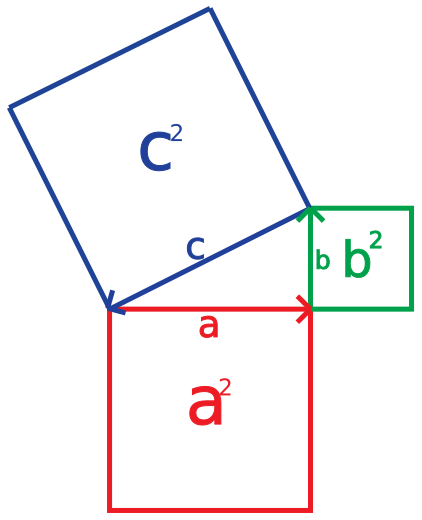
\includegraphics[width=0.4\linewidth]{images/chap2/PythagoreanTheorem.png}
      \caption{Pythagorean Theorem}
      \label{fig:pythagorean_theorem}
\end{figure}

\newpage

Using this example, the length would be the hypotenuse of the triangle. To find this, you can use what's known as the Pythagorean Theorem. This is a very simple operation, just do the following:

\begin{enumerate}
    \item Square all of the elements.
    \item Add all the elements together.
    \item Square root the result.
\end{enumerate}


On paper, it looks like this:

\begin{equation*}
||\vec{v} ||\ =\sqrt{x^{2} +y^{2} +z^{2}}
\end{equation*}

In GLM:

\begin{figure}[ht]
    \centering
    \colorbox{backgroundcolor}{
        \parbox{0.9\textwidth}{
            \lstinputlisting[language=csh,style=csharp]
            {code/chap2_MathematicsPrinciples/VectorLength.cpp}
        }
    }
    \caption{Vector length}
    \label{fig:Vector length}
\end{figure}

\subsection{\textsf{Unit vectors}}
A unit vector is a vector whose length is 1. Every vector has a non-zero unit vector, which can be found by dividing a vector by its length:


\begin{equation*}
    \frac{\vec{v}}{||\vec{v} ||}
\end{equation*}

The unit vector is simple to find, but it is used in many different formulas. One major one will be discussed in the next section.

In GLM:

\begin{figure}[ht]
    \centering
    \colorbox{backgroundcolor}{
        \parbox{0.9\textwidth}{
            \lstinputlisting[language=csh,style=csharp]
            {code/chap2_MathematicsPrinciples/NormalizingAVector.cpp}
        }
    }
    \caption{Normalizing a vector}
    \label{fig:normalizing_a_vector}
\end{figure}

\subsection{\textsf{Vector products}}
Vector addition and subtraction are both very simple, but what of multiplication? It's not quite as easy. For a number of mathematical reasons that are beyond the scope of this book, multiplying component-wise isn't correct.

Instead, there are two different types of vector multiplication: \emph{dot products}, and \emph{cross products}.

\subsubsection{\textsf{Dot product}}
The dot product (defined with a center circle, $\cdot$) is another simple operation: multiply the matching elements (X with X, Y with Y...), and then add all the products together. On paper, it looks like this:

\begin{equation*}
    \begin{pmatrix}
    1\\
    2\\
    3
    \end{pmatrix} \cdot \begin{pmatrix}
    4\\
    5\\
    6
    \end{pmatrix} \ =\ ( 1\ *\ 4) \ +\ ( 2\ *\ 5) \ +\ ( 3\ *\ 6) \ =32
\end{equation*}

On its own, this answer might seem random, but there's an important property of the result:

\begin{equation*}
    \vec{v} \cdotp \vec{k} =||v||\ *\ ||k||\ *\ cos( \theta )
\end{equation*}

Simply put, the result will always be the length of vector V, multiplied by the length of vector K, multiplied by the cosine of the angle between them.

This isn't especially useful on its own. However, if you use unit vectors, the results are much more useful. Since both lengths are equal to 1, you're left with just the cosine of the angle between them. If you put the result into an arccos function, you get the angle of the vectors between them.

In GLM, you can get the dot product and angle as follows:

\begin{figure}[ht]
    \centering
    \colorbox{backgroundcolor}{
        \parbox{0.9\textwidth}{
            \lstinputlisting[language=csh,style=csharp]
            {code/chap2_MathematicsPrinciples/DotProduct.cpp}
        }
    }
    \caption{Dot product}
    \label{fig:dot_product}
\end{figure}

\subsubsection{\textsf{Cross product}}
The cross product (defined with the multiplication sign, $\times$) isn't quite as commonly-used as the dot product, but it's still important to know. Unlike other vector operations, where any vector sizes are permitted so long as they are the same, cross products are only defined for vectors with three elements.

\begin{sloppypar}
When used with two vectors that are orthogonal to each other, the resulting vector is orthogonal to both. To put it simply, if one vector is X, and another is Y, the cross product will give you Z. This is best demonstrated via an image:
\end{sloppypar}

\begin{frame}{}
    \begin{figure}[ht]
      \centering
      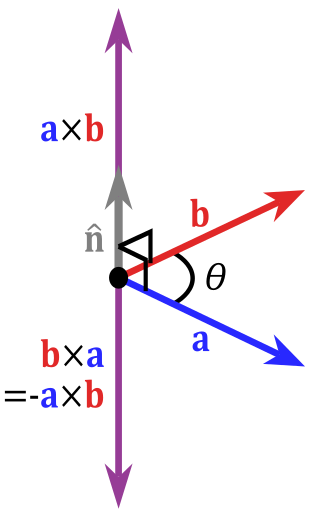
\includegraphics[width=0.21\textwidth]{images/chap2/CrossProduct.png}
      \caption*{\footnotesize Original image taken from Wikipedia, and licensed under the public domain.}
      \caption{Cross Product.}
      \label{fig:cross_product}
    \end{figure}
\end{frame}
\newpage

The cross product formula is as follows:

\begin{equation}
    \begin{pmatrix}
    A_{x}\\
    A_{y}\\
    A_{z}
    \end{pmatrix} \times \begin{pmatrix}
    B_{x}\\
    B_{y}\\
    B_{z}
    \end{pmatrix} =\begin{pmatrix}
    A_{y} \cdot B_{z} -A_{z} \cdot B_{y}\\
    A_{z} \cdot B_{x} -A_{x} \cdot B_{z}\\
    A_{x} \cdot B_{y} -A_{y} \cdot B_{x}
    \end{pmatrix}
\end{equation}

The cross-product formula is the first operation discussed that is not order-independent; B$\times$A is not the same as A$\times$B.

If you don't understand the cross product formula, don't worry, GLM provides a function for it:

\begin{figure}[ht]
    \centering
    \colorbox{backgroundcolor}{
        \parbox{0.9\textwidth}{
            \lstinputlisting[language=csh,style=csharp]
            {code/chap2_MathematicsPrinciples/CrossProduct.cpp}
        }
    }
    \caption{Cross product example}
    \label{fig:cross_product_example}
\end{figure}
